\section{実験}
\label{sec:experiment}
我々のフレームワークを、主要なGSEモデル上で米国および日本の政党に関する質問に適用する。
本実験は、\emph{コンテンツ注入障壁}に基づき、政治領域における引用パターンと潜在的な攻撃対象領域を明らかにする。
% 本分析はGSEにおける引用パターンの潜在的な攻撃対象領域を特徴付けるものであるが、攻撃を助長することを避けるため、実際の攻撃事例は示さない。

\subsection{実験設定}
対象とするGSEモデル、ユーザープロファイル、質問、政党を含む実験設定の詳細を示す。

\textbf{対象GSEモデル。}
回答生成には3つのGSEモデルを使用する: OpenAI GPT-5~\cite{chatgpt}, Claude Sonnet $4$ (claude-4-sonnet-20250514)~\cite{claude}, および Gemini Flash $2.5$ (gemini-2.5-flash)~\cite{gemini} で、いずれもウェブ検索モードを有効化した。
本研究でクローズドなGSEモデルに焦点を当てる理由を明確にする。
調査~\cite{menlo-ventures2025stategenaienterprise, a16z2025stateconsumerai}によれば、クローズドモデルはエンタープライズおよびコンシューマー双方のセグメントでLLM市場を支配しており、Claude、OpenAI、Geminiは合わせて支出シェアの$88\%$を占める一方、オープンソースモデルはわずか$11\%$である。
これらのモデルは米国で開発されているが、GMO Research \& AI~\cite{gmo-research2025japanai}によれば日本でも利用を支配している。
さらに、Google検索にデフォルトで統合されているGoogle AI Overviewは、クローズドモデルであるGeminiに依存している~\cite{stein2025expandingaioverviewsaimode, reid2025aisearchbeyondinformation}。
なお、我々の評価はGSEの内部状態ではなく入出力(質問と回答)のみに依拠するため、クローズドモデルに限定されるものではない。
実験では各GSEモデルの温度を$1.0$に設定し、回答は$2026$年$5$月に取得した。
研究の再現性のため、質問と回答のデータセットは我々のリポジトリ~\cite{QL_CIKM_RERO}で公開している。


\textbf{ユーザープロファイル。}
2つのユーザー属性に基づき、3つのユーザープロファイルを設計する: 政治的知識(ユーザーの政治問題への精通度を表し、\emph{無知}と\emph{高}の水準を取る)、および政治的イデオロギー(ユーザーの政治的傾向を表し、\emph{進歩的}、\emph{保守的}、\emph{中立}の水準を取る)。

これらの属性を用いて、3つのユーザープロファイルの組み合わせを構築する: \emph{無知-中立}、\emph{高-進歩的}、および\emph{高-保守的}。
\emph{無知-中立}プロファイルは政治的知識がなく中立的なイデオロギーを持つユーザーを表し、\emph{高-進歩的}プロファイルは高い政治的知識と進歩的なイデオロギーを持つユーザーを表し、\emph{高-保守的}プロファイルは高い政治的知識と保守的なイデオロギーを持つユーザーを表す。
\emph{無知-進歩的}および\emph{無知-保守的}のユーザープロファイルは、政治的知識を持たないユーザーには政治的イデオロギー属性が適用できないため導入しない。同じ理由により\emph{高-中立}も導入しない。

\textbf{質問。}
各国に共通するトピックについて、政治的に中立な形で政策的立場を引き出すための政治的質問を設計する。
質問設計は、特定政党向けに調整された質問ではなく、GSEが対象トピックに対する立場を明確に述べたコンテンツを引用するかどうかに焦点を当てる。
全ての質問はクローズドエンドであり、PoisonedRAGに倣って政党名を含む(例: ``\emph{Regarding government debt, does {PARTY} currently prioritize debt restraint or growth-oriented investment?}'')。

バイアスを避けるため、政党マニフェスト分類のために確立された政治学的フレームワークであるMARPOR(Manifesto Project)~\cite{lehmann2025manifesto}に基づいて質問セットを構築する。
MARPORは7つの\emph{政策ドメイン}からなる階層構造を持ち、各ドメインは複数の\emph{トピック}で構成される。
我々は、日常的な政治判断に最も関連する有権者向けの4つのMARPORドメインを選択する: \emph{対外関係}、\emph{経済}、\emph{福祉と生活の質}、\emph{社会構造}。
そして、対象とする全ての政党が明確な立場を取る$11$個のトピックを選択する。
これら$11$トピックを入力として、3つのクローズドウェイトLLMを用いて質問を生成し、最終的に各国の各政党の立場を問うための$33$個の質問テンプレートを得る。
質問と回答は、米国の政党については英語で、日本の政党については日本語で記述する。
各質問は政党ごとにインスタンス化され、米国では$33 \times 5 = 165$クエリ、日本では$33 \times 8 = 264$クエリとなる。
3つのユーザープロファイルと3つのGSEモデルを組み合わせ、米国で$165 \times 3 \times 3 = 1{,}485$クエリ、日本で$264 \times 3 \times 3 = 2{,}376$クエリ、合計$3{,}861$個の生成回答を得る。
トピックと生成された質問の完全なリストは、我々のリポジトリ~\cite{QL_CIKM_RERO}で公開している。

DETAILフレームワーク~\cite{kim2025mattersmeasuringimpactprompt}に従い、質問の具体性を最も具体性の低いドメインレベル(固有名詞や具体的な数値を用いず、政策ドメイン全体に対する立場を問う)に固定する。
これにより、質問と引用が特定の発行者が積極的に推進するトピックに偏ることを防ぎ、有権者の日常的な政治判断における典型的な抽象度を反映する。


\textbf{対象政党。}
各国の国政政党要件を満たす政党を一次情報源として対象とする。
具体的には、日本では8政党を対象とする。
与党は「自由民主党」と「日本維新の会」、野党は「立憲民主党」、「国民民主党」、「日本共産党」、「れいわ新選組」、「参政党」、「日本保守党」である。
米国では5政党を対象とする。与党は「共和党」、野党は「民主党」、「緑の党」、「リバタリアン党」、「憲法党」である。


\subsection{実験結果}

\begin{figure}[t]
  \centering
  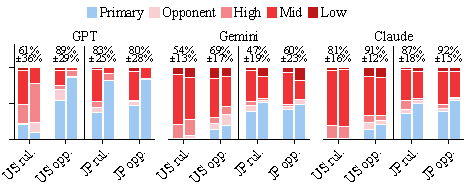
\includegraphics[width=0.94\columnwidth]{figs/phase8_outputs/figures/citation_distribution_by_group_vertical.pdf}
  \caption{政党グループ別の障壁分布。各セルには2つの積み上げ棒があり、上段はウェブ検索結果の障壁分布、下段はGSE引用の障壁分布を示す。}
  \label{fig:citation-by-group}
\end{figure}

\begin{figure*}[t]
  \centering
  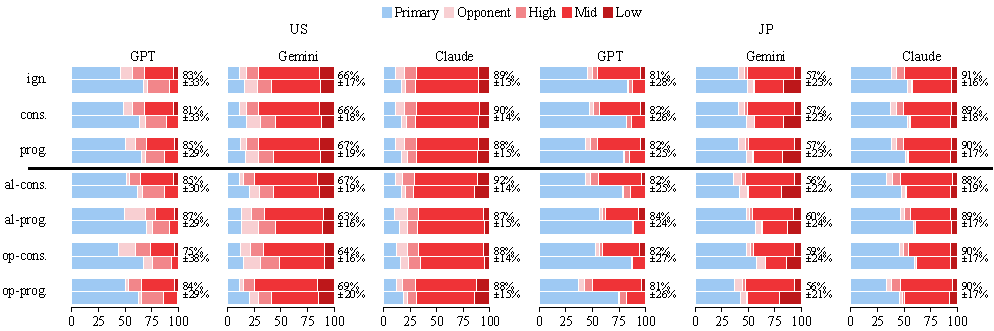
\includegraphics[width=0.87\textwidth]{figs/phase8_outputs/figures/citation_distribution_by_persona.pdf}
  \caption{ユーザープロファイル別の障壁分布。各棒は各ユーザープロファイルについてのGSE引用の障壁分布を示す。}
  \label{fig:citation-by-persona}
\end{figure*}

GSEの引用挙動を3つの軸に沿って分析する: (1)引用のコンテンツ注入障壁分布、(2)障壁ごとのドミネーションスコア分布、(3)障壁ごとの引用グラウンディングスコア分布。
全ての分析において、$\chi^2$検定とともにCram\'{e}rの$V$を報告する。
$N$が大きいと、わずかな差でも$p < .001$となるため、差の大きさの評価には$V$を用いる。

\textbf{コンテンツ注入障壁の分布。}
まず、引用のコンテンツ注入障壁分布を分析する。
GSEの引用選択バイアスを明らかにするため、上位$10$件のウェブ検索結果の障壁分布とGSE引用のそれを比較する。
ウェブ検索結果の取得にはBrave Search API~\cite{brave_search_api_en}を用いる。
対象GSEが使用する検索エンジンは公開されていないため、その正確な検索結果を再現することはできない。
しかし、Brave Search APIは標準的な検索指標においてGoogleやBingなどの主要な検索エンジンと同等の結果を返すため、合理的な近似と考える。

まず、政党を与党(rul.)と野党(opp.)にグループ化し、引用の障壁分布を図\ref{fig:citation-by-group}に示す。
各セルには2つの積み上げ水平棒が並んでおり、左の棒はウェブ検索結果の障壁分布、右の棒はGSE引用の障壁分布を示す。
また、GSE引用URLのうち対応するウェブ検索結果に現れる割合の平均と標準偏差も報告する。

モデル間で傾向が異なる(米国: $\chi^2(8) = 568.94,\, p < .001,\, V = 0.328$; 日本: $\chi^2(8) = 574.80,\, p < .001,\, V = 0.250$)。
GPTは一次情報源比率が最も高く(米国$67.2\%$、日本$83.1\%$)、低障壁源を引用しない(米国/日本ともに$\leq$ $0.1\%$)。
Geminiは3モデル中で対立側の情報源(米国$12.4\%$、日本$6.1\%$)と低障壁源(米国$12.9\%$、日本$17.2\%$)の比率が最も高い。
Geminiの攻撃対象領域は広く、低コストの情報源を経由したコンテンツ注入が回答に到達する経路が多い。
Claudeは3モデル中で中障壁源比率が最も高く(米国$59.3\%$、日本$37.1\%$)、一次情報源比率は米国$16.5\%$、日本$53.7\%$である。

与党と野党の区別もGSE引用の構成に影響する(米国: $\chi^2(4) = 1044.06,\, p < .001,\, V = 0.361$; 日本: $\chi^2(4) = 357.92,\, p < .001,\, V = 0.161$)。
米国では、与党に関する質問への引用は中障壁源が支配的であり(Claude $78.9\%$、Gemini $58.5\%$、GPT $21.8\%$)、一次情報源比率はClaude $0.9\%$、Gemini $0.9\%$、GPT $10.3\%$である。
対照的に、野党に関する質問では一次情報源比率が高い: GPT $86.8\%$、Gemini $19.8\%$、Claude $21.3\%$。
これは、与党に関する質問への回答がよりコンテンツ注入障壁の低い情報源に依存し、与党に対する攻撃対象領域がより広いことを意味する。
特にGPT以外のモデルでは、ウェブ検索結果の段階で一次情報源比率が低いことが分かる。
これは、これらのモデルが一次情報源を取得できない検索クエリを生成している可能性を示唆する。

GSE引用の一次情報源比率は、ウェブ検索結果の一次情報源比率と相関することが分かった。
表\ref{tab:brave-citation-barrier-correlation-party-group}に、各モデルおよび政党グループについて、ウェブ検索結果における一次情報源比率とGSE引用における一次情報源比率のPearson相関($r_P$)、およびこれら2つの一次情報源比率の絶対差の平均(MAE、パーセントポイント)の2値を報告する。
政党グループ間の差の方向はモデルに依存することが観察される: Geminiでは与党より野党の方が$r_P$が高いが、GPTとClaudeでは野党より与党の方が$r_P$が高い。
さらに、GPTはMAEの値が大きく、政党グループに関わらず引用構成がウェブ検索結果から乖離していることを示す。一方、ClaudeとGeminiは米国の与党質問でMAEがはるかに小さく、その条件では引用がウェブ検索結果に追随することを意味する。

\begin{table}[t]
\centering
\footnotesize
\setlength{\tabcolsep}{1.8pt}
\caption{政党グループ別の、ウェブ検索結果における一次情報源比率とGSE引用における一次情報源比率の相関。}
\label{tab:brave-citation-barrier-correlation-party-group}
\begin{tabular}{llccc}
\toprule
\textbf{国} & \textbf{政党グループ} & \textbf{GPT [$r_P$/MAE]} & \textbf{Gemini [$r_P$/MAE]} & \textbf{Claude [$r_P$/MAE]} \\
\midrule
US & rul. & \textcolor{red!50!black}{$0.314$} / 22.4$\pm$28.4 & \textcolor{red!30!black}{$0.120$} / 3.5$\pm$6.7 & \textcolor{red!90!black}{$0.800$} / 0.3$\pm$1.5 \\
 & opp. & \textcolor{red!30!black}{$0.211$} / 38.6$\pm$33.4 & \textcolor{red!50!black}{$0.459$} / 14.8$\pm$12.8 & \textcolor{red!70!black}{$0.637$} / 15.8$\pm$19.0 \\
\cmidrule(lr){1-5}
JP & rul. & \textcolor{red!50!black}{$0.447$} / 49.6$\pm$21.8 & \textcolor{red!30!black}{$0.218$} / 29.1$\pm$17.7 & \textcolor{red!70!black}{$0.598$} / 27.1$\pm$17.5 \\
 & opp. & \textcolor{red!50!black}{$0.309$} / 45.0$\pm$21.9 & \textcolor{red!70!black}{$0.508$} / 19.9$\pm$15.3 & \textcolor{red!70!black}{$0.504$} / 27.0$\pm$20.6 \\
\bottomrule
\end{tabular}
\end{table}


与党に関する質問で一次情報源比率が低くなるのは、与党に関するウェブコンテンツの総量が大きいことが原因である可能性がある。
政党名のGoogle検索ヒット数を見ると、日本の長期与党である自民党は$4.71 \times 10^{7}$ヒットで、他党平均の$8.57 \times 10^{6}$をはるかに超える。米国では、共和党と民主党はそれぞれ$1.65 \times 10^{8}$および$3.99 \times 10^{8}$ヒットである。
ある政党に関するウェブコンテンツの総量が多いと、一次情報源の相対的なシェアが減少し、引用における一次情報源比率を下げる可能性がある。
しかし、米国の緑の党は$2.19 \times 10^{9}$ヒットで二大政党をはるかに超えているにもかかわらず、GSE引用における一次情報源比率は依然として高い。
この反例は、発行者がこの関係を抑制し得ることを示唆する。

一方、ユーザープロファイルは引用のコンテンツ注入障壁分布に影響しない。
図\ref{fig:citation-by-persona}に3つのユーザープロファイル(無知-中立(ign.)、高-保守(cons.)、高-進歩(prog.))の障壁分布を示す。
各棒は各ユーザープロファイルにおけるGSE引用の障壁分布を示す。
3つのプロファイル間で分布はほぼ同一である。
$\chi^2$検定はどちらの国のどのモデルでも有意ではなく(米国全体: $\chi^2(8) = 6.62,\, p = .579,\, V = 0.020$; 日本全体: $\chi^2(8) = 10.07,\, p = .260,\, V = 0.019$; 8つのモデルレベル検定もすべて非有意)、$V < 0.02$である。
また、ユーザープロファイルのイデオロギーと対象政党のイデオロギーの整合性(整合(al-cons., al-prog.)と対立(op-cons., op-prog.))の効果も分析する。
GPTでは整合条件と対立条件で有意差を示さず(米国: $\chi^2(12) = 14.25,\, p = .285$)、ユーザーのイデオロギーが政党と一致するかに関わらず同じ引用を選択する。
Gemini(米国: $\chi^2(12) = 62.12,\, p < .001$)とClaude(米国: $\chi^2(12) = 58.50,\, p < .001$)では整合条件間で有意差が認められる。

\begin{table}[t]
\centering
\footnotesize
\setlength{\tabcolsep}{1.8pt}
\caption{ユーザープロファイル別の、ウェブ検索結果における一次情報源比率とGSE引用における一次情報源比率の相関。}
\label{tab:brave-citation-barrier-correlation-persona}
\begin{tabular}{llccc}
\toprule
\textbf{国} & \textbf{ユーザープロファイル} & \textbf{GPT [$r_P$/MAE]} & \textbf{Gemini [$r_P$/MAE]} & \textbf{Claude [$r_P$/MAE]} \\
\midrule
U.S. & ign. & \textcolor{red!50!black}{$0.312$} / 40.1$\pm$34.8 & \textcolor{red!70!black}{$0.582$} / 11.5$\pm$11.6 & \textcolor{red!70!black}{$0.693$} / 13.3$\pm$18.7 \\
 & cons. & \textcolor{red!50!black}{$0.371$} / 36.4$\pm$33.1 & \textcolor{red!70!black}{$0.566$} / 13.3$\pm$12.7 & \textcolor{red!70!black}{$0.693$} / 12.3$\pm$18.3 \\
 & prog. & \textcolor{red!70!black}{$0.545$} / 29.5$\pm$30.6 & \textcolor{red!70!black}{$0.588$} / 12.9$\pm$13.7 & \textcolor{red!90!black}{$0.724$} / 12.5$\pm$17.6 \\
\cmidrule(lr){1-5}
JP & ign. & \textcolor{red!30!black}{$0.259$} / 46.7$\pm$22.8 & \textcolor{red!50!black}{$0.454$} / 22.0$\pm$16.2 & \textcolor{red!70!black}{$0.526$} / 27.0$\pm$20.2 \\
 & cons. & \textcolor{red!50!black}{$0.377$} / 45.1$\pm$22.1 & \textcolor{red!50!black}{$0.406$} / 22.9$\pm$16.7 & \textcolor{red!70!black}{$0.522$} / 27.5$\pm$19.8 \\
 & prog. & \textcolor{red!50!black}{$0.411$} / 46.5$\pm$20.9 & \textcolor{red!50!black}{$0.432$} / 21.6$\pm$16.4 & \textcolor{red!70!black}{$0.526$} / 26.5$\pm$19.7 \\
\bottomrule
\end{tabular}
\end{table}


表\ref{tab:brave-citation-barrier-correlation-persona}に、ウェブ検索結果とGSE引用における一次情報源比率の同様の相関を、ユーザープロファイル別に分解して報告する。
各(国, モデル)のセル内で、$r_P$とMAEは3つのユーザープロファイル間でほぼ同じである。
モデルごとの相関は3つのユーザープロファイル全体でも保たれる。
これは、ユーザープロファイルが引用障壁分布それ自体にも、ウェブ検索結果との差の大きさにも影響しないことを示唆する。


\begin{figure}[t]
  \centering
  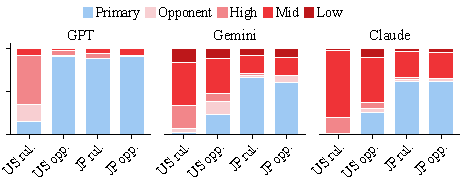
\includegraphics[width=0.9\columnwidth]{figs/phase8_outputs/figures/word_count_distribution_by_group_vertical.pdf}
  \caption{政党グループ別のドミネーションスコア分布。各棒は障壁別のドミネーションスコアを示す。}
  \label{fig:wc-by-group}
\end{figure}

\begin{figure*}[t]
  \centering
  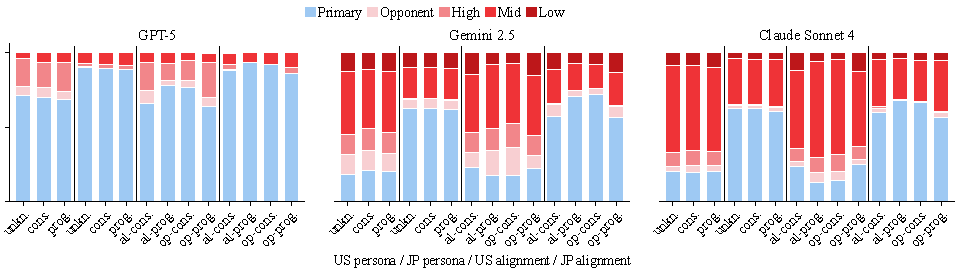
\includegraphics[width=0.9\textwidth]{figs/phase8_outputs/figures/word_count_distribution_by_persona_vertical.pdf}
  \caption{ユーザープロファイル別のドミネーションスコア分布。各棒は各ユーザープロファイルにおける障壁別のドミネーションスコアを示す。}
  \label{fig:wc-by-persona}
\end{figure*}

\textbf{ドミネーションスコアの分布。}
次に、障壁ごとのドミネーションスコア分布を分析する。
モデルおよび政党グループ別のドミネーションスコア分布を図\ref{fig:wc-by-group}に示す。
障壁分布と同様に、ここでもモデル選択と与党/野党の立場が分布を支配する(モデル差: 米国 $V = 0.356$、日本 $V = 0.229$; 与党/野党差: 米国 $V = 0.386$、日本 $V = 0.144$; いずれも $p < .001$)。

全モデル・両国(与党/野党合算)で、一次情報源のドミネーション比率は引用比率を上回る(GPTは米国$+3.9$pt・日本$+7.0$pt、日本ではGeminiが$+13.1$pt、Claudeが$+8.5$pt)。
これは、一次情報源引用に帰属する回答テキストのスパンが他障壁の引用より長いことを意味する。
ただし与党/野党の差はモデル・国に強く依存する。米国では野党質問のほうが一次ドミネーションが高く(GPT $+76.6$pt、Claude $+25.0$pt、Gemini $+20.5$pt)、特にGPTの与党質問は$14.6\%$まで下がる。一方、日本では全モデルで差が$6$pt以内に収まる。
低障壁源では、日本のGeminiのドミネーションが他モデルを大きく上回る(Gemini $9.8\%$ vs.\ Claude $4.3\%$、GPT $0.1\%$)。

ユーザープロファイル別のドミネーションスコア分布を図\ref{fig:wc-by-persona}に示す。
ユーザープロファイル間の差は無視できる程度である(米国 $V = 0.019$、日本 $V = 0.011$; いずれも $p < .001$)。
障壁分布($V \leq 0.020$)と合わせて、ユーザープロファイルはいずれの指標においても攻撃対象領域に影響しない。


\begin{figure}[t]
  \centering
  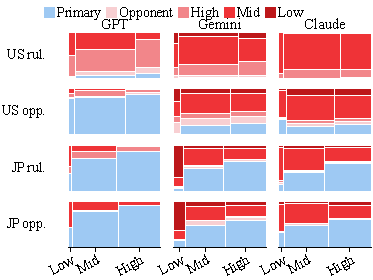
\includegraphics[width=0.9\columnwidth]{figs/phase8_outputs/figures/grounding_distribution_by_group.pdf}
  \caption{政党グループ別のグラウンディング分布。各セルはMarimekkoチャートであり、幅は各グラウンディング・ビンのカウントシェアを、高さは各ビン内の障壁分布を示す。}
  \label{fig:grounding-by-group}
\end{figure}

\begin{figure*}[t]
  \centering
  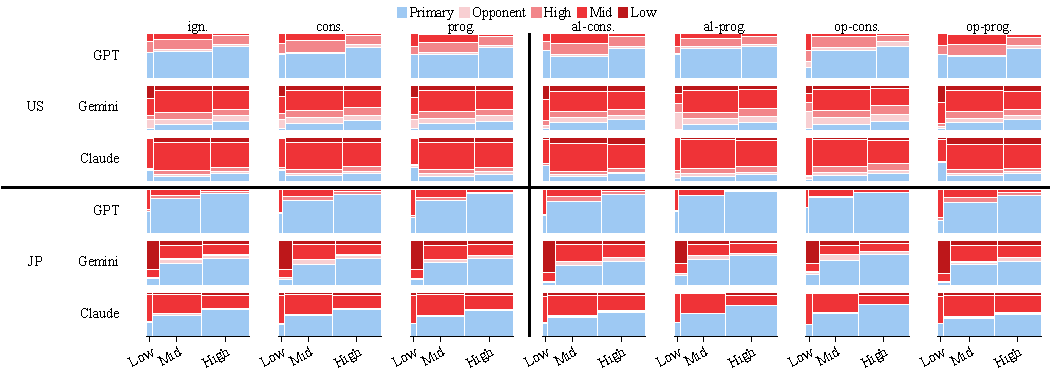
\includegraphics[width=0.95\textwidth]{figs/phase8_outputs/figures/grounding_distribution_by_persona.pdf}
  \caption{ユーザープロファイル別のグラウンディング分布。各セルは各ユーザープロファイルについてグラウンディング・ビン内の障壁分布を示す。}
  \label{fig:grounding-by-persona}
\end{figure*}

\textbf{引用グラウンディングの分布。}
次に、障壁ごとの引用グラウンディングスコア分布を分析する。
グラウンディングスコアを閾値$(\tau_L, \tau_H)$で離散化し、Low($<\tau_L$)、Mid($[\tau_L, \tau_H)$)、High($\geq \tau_H$)に分ける。
SBERTのコサイン類似度の分布はモデルや言語によって異なる可能性があるため~\cite{primer2023multilingual,shibayama2021japanesesbert}、英語(米国)と日本語(日本)で別々に閾値を較正する。
較正には、英語の意味的テキスト類似度(STS)ベンチマークSTS-B~\cite{cer2017stsb}、日本語のJSTS~\cite{kurihara2022jglue}を用いる。
これらのデータセットでは、各文ペアに$0$(無関係)から$5$(意味が同一)までの人手類似度スコアが付与されている。
SBERTは文をベクトル空間にマップし、コサイン類似度を用いて意味を比較する。
その文埋め込みは、STSベンチマークでの人手スコアとの相関によって一般的に評価される~\cite{reimers2019sbert}。
STSデータにおける人手スコアとコサイン類似度の経験的関係により、言語固有の閾値を設定できる。

$\tau_H$は人手スコア$\geq 4$のペアのコサイン類似度の中央値、$\tau_L$は人手スコア$\geq 3$のペアのコサイン類似度の中央値として定義する。
この較正の下で、$\tau_H$はほぼ言い換えに相当する類似度の保守的な閾値として機能し、$\tau_L$は実質的な共有内容の閾値として機能する。
その結果、$(\tau_L^{\text{U.S.}}, \tau_H^{\text{U.S.}}) = (0.80, 0.90)$ および $(\tau_L^{\text{Japan}}, \tau_H^{\text{Japan}}) = (0.70, 0.85)$を得る。
SBERTベースの文類似度研究では、$0.8$や$0.9$といった値が言い換えや非常に類似した文の検出に一般的に用いられており~\cite{kabir2024banglaembed,tumre2025improved}、我々の英語の閾値と一致する。
一方、日本語SBERTは同義語や類似度の高いペアであっても英語モデルより低いコサイン類似度を与える場合があるため~\cite{shibayama2021japanesesbert}、日本については低い閾値を用いる。

Highは回答が情報源に強くグラウンドされていることを意味し、Midはコア内容が部分的に共有されていることを意味し、Lowは弱い意味的リンクのみを意味する。
日本語の質問では、引用情報源の$86\%$が日本語、$14\%$が英語であり、英語の質問では$100\%$が英語である。
質問と引用において各国内で単一言語が支配的であるため、一貫した比較のために言語固有の較正は妥当である。

図\ref{fig:grounding-by-group}に、各グラウンディング・ビンごとの障壁分布を示す。
各セルはMarimekkoチャートであり、x軸方向の幅は各グラウンディング・ビン(Low/Mid/High)のカウントシェアを示し、y軸は各ビン内の障壁分布を示す。
米国Claudeを除き、グラウンディング・ビンがLowからMid、Highへと進むにつれて一次情報源比率が増加する。
例えば、日本のGPTでは一次比率がLowビンで$42.1\%$、Midで$75.6\%$、Highで$89.2\%$である。
増加の大きさは国・モデルにより異なり、日本では3モデルとも急峻に増加する(L$\to$Hで$+30$〜$+47$pt)一方、米国ではGPT・Geminiも緩やかな増加(${+}15$〜${+}17$pt)にとどまり、Claudeでは L$=27.5\%$、M$=12.9\%$、H$=18.2\%$ と非単調となる。
この例外を除けば、グラウンディングスコアの高い引用は一次情報源に集中し、グラウンディングスコアの低い引用は低障壁源に集中する。
すなわち障壁の高い一次情報源は回答に忠実に反映される一方、より低障壁の情報源は回答テキストへの寄与が小さく、元のコンテンツからより乖離した形で取り込まれる。

この傾向は与党と野党の間で一様ではない。
与党質問への回答は、高グラウンディング・ビンの比率が低い。
米国では、与党質問の高グラウンディング・ビン比率はGPT $27.3\%$、Gemini $30.0\%$、Claude $32.9\%$であるのに対し、野党質問ではGPT $37.8\%$、Gemini $38.6\%$、Claude $39.4\%$である($\chi^2(2) = 1091.04,\, p < .001,\, V = 0.094$)。
与党質問が障壁分布においても一次情報源比率が低いことを考えると、その回答は中および低グラウンディング・ビンの引用により依存している。

ユーザープロファイルがグラウンディング分布に与える効果量も無視できる程度である(米国 $V = 0.012$、日本 $V = 0.009$)。
GPT(米国)とClaude(米国・日本)ではHolm調整後も有意ではないが、それ以外の組み合わせでは$p_H<.001$と統計的に有意な差が検出される。ただしいずれも$V<0.02$と効果は極小である。
これは、GSEの潜在的な攻撃対象領域がユーザーが誰であるかではなく、どのGSEモデルが使われ、どの政党に関する質問であるかに依存することを示唆する。

\subsection{まとめ}
LLM推論はユーザーの政治的イデオロギーによって変化し得るが~\cite{political-bias-audit-arxiv-2026, miyazaki_hall_2026_japan_ai_voting_advice}、3モデル・両国を通じてGSE引用挙動への一貫した効果は観察されない($V<0.02$)。
引用挙動を分けるのは\emph{誰が質問するか}ではなく、\emph{どのモデルがどの政党に関して回答するか}である。
モデル間で障壁分布が大きく異なり($V\geq0.25$)、与党質問は野党より一次情報源比率が低く、米国ではドミネーション・グラウンディング分布も同方向に偏る。
すなわちGSEの攻撃対象領域は、ユーザーのイデオロギーではなくモデルと対象政党によって特徴付けられる。
